\section{ttH process\footnote{C.~Collins-Tooth, C.~Neu, L.~Reina,
M.~Spira (eds.); S.~Dawson, S.~Dean, S.~Dittmaier, M.~Kr\"amer,
C.T.~Potter and D.~Wackeroth.}}

%\vskip 0.8cm

%\noindent
%{\sc C.~Collins-Tooth$^1$, S.~Dawson$^2$, S.~Dean$^3$,
%S.~Dittmaier$^4$, M.~Kr\"amer$^5$, C.~Neu$^6$, C.T.~Potter$^7$,
%L.~Reina$^8$, M.~Spira$^9$ and D.~Wackeroth$^{10}$}

%\vskip 0.8cm

%\begin{small}
%\noindent
%{\it \small
%$^1$ University of Glasgow, Department of Physics and Astronomy, Glasgow
%G12 8QQ, United Kingdom \\
%$^2$ Department of Physics, Brookhaven National Laboratory, Upton, NY
%11973, USA \\
%$^3$ University College London, Department of Physics and Astronomy,
%Gower Street, London WC1E 6BT, United Kingdom \\
%$^4$ Physikalisches Institut, Albert-Ludwigs-Universit\"at Freiburg,
%D--79104 Freiburg, Germany \\
%$^5$ Institut f\"ur Theoretische Physik, RWTH Aachen University,
%D--52056 Aachen, Germany \\
%$^6$ University of Virginia, Charlottesville, VA 22906, USA \\
%$^7$ University of Oregon, Center for High Energy Physics, Eugene, OR
%97403-1274, USA \\
%Street, Montreal, Quebec H3A 2T8, Canada \\
%$^8$ Physics Department, Florida State University, Tallahassee, FL
%32306-4350, USA \\
%$^9$ Paul Scherrer Institut, CH--5232 Villigen PSI, Switzerland \\
%$^{10}$ Department of Physics, SUNY at Buffalo, Buffalo, NY 14260-1500, USA}
%\end{small}
%
%\vskip 0.8cm

\subsection{Higgs-boson production in association with $\PQt\PAQt$ pairs}
%           ============================================================
Higgs radiation off top quarks $\PQq\PAQq/\Pg\Pg\to \PH\PQt\PAQt$ (see
\Fref{fg:lodiatth}) plays a role for light Higgs masses below $\sim
150$ \UGeV\ at the LHC. The measurement of the $\PQt\PAQt\PH$ production
rate can provide relevant information on the top--Higgs Yukawa coupling.
The leading-order (LO) cross section was computed a long time ago
\cite{Raitio:1978pt,Ng:1983jm,Kunszt:1984ri,Gunion:1991kg,Marciano:1991qq}.
These LO results are plagued by large theoretical uncertainties due to
the strong dependence on the renormalization scale of the strong
coupling constant and on the factorization scales of the parton
density functions inside the proton, respectively. For the LO cross
section there are several public codes available, as e.g.\ {\sc HQQ}
\cite{Spira:1997dg,HQQ}, {\sc Madgraph/Madevent}
\cite{Stelzer:1994tk,Madgraph}, {\sc MCFM} \cite{MCFM}, or {\sc PYTHIA}
\cite{PYTHIA}.  The dominant background processes for this signal
process are $\PQt\PAQt\PQb\PAQb$, $\PQt\PAQt jj$, $\PQt\PAQt\PGg\PGg$,
$\PQt\PAQt\PZ$, and $\PQt\PAQt\PWp\PWm$
production depending on the final-state Higgs-boson decay.
\begin{figure}[htb]
\begin{center}
\SetScale{0.8}
\begin{picture}(130,90)(0,0)
\ArrowLine(0,100)(50,50)
\ArrowLine(50,50)(0,0)
\Gluon(50,50)(100,50){3}{5}
\ArrowLine(100,50)(120,70)
\ArrowLine(120,70)(150,100)
\ArrowLine(150,0)(100,50)
\DashLine(120,70)(150,70){5}
\Vertex(50,50){2}
\Vertex(100,50){2}
\Vertex(120,70){2}
\put(-12,78){$\PQq$}
\put(-12,-2){$\PAQq$}
\put(125,53){$\PH$}
\put(125,78){$\PQt$}
\put(125,-2){$\PAQt$}
\end{picture}
\begin{picture}(130,90)(-80,0)
\Gluon(0,0)(50,0){3}{5}
\Gluon(0,100)(50,100){3}{5}
\ArrowLine(100,0)(50,0)
\ArrowLine(50,0)(50,50)
\ArrowLine(50,50)(50,100)
\ArrowLine(50,100)(100,100)
\DashLine(50,50)(100,50){5}
\Vertex(50,100){2}
\Vertex(50,50){2}
\Vertex(50,0){2}
\put(85,35){$\PH$}
\put(-12,78){$\Pg$}
\put(-12,-2){$\Pg$}
\put(85,78){$\PQt$}
\put(85,-2){$\PAQt$}
\end{picture}
\end{center}
\caption[]{Examples of LO Feynman diagrams for the
partonic processes $\PQq\PAQq,\Pg\Pg\to\PQt\PAQt\PH$.}
\label{fg:lodiatth} 
\end{figure}

The full next-to-leading-order (NLO) QCD corrections to $\PQt\PAQt\PH$
production have been calculated
\cite{Beenakker:2001rj,Beenakker:2002nc,Reina:2001sf,Dawson:2002tg}
resulting in a moderate increase of the total cross section at the LHC
by at most $\sim 20\%$, depending on the value of $\MH$ and on the PDF
set used. Indeed, when using CTEQ6.6 the NLO corrections are always
positive and the $K$-factor varies between $1.14$ and $1.22$ for
$\MH=90,\ldots,300\UGeV$, while when using MSTW2008 the impact of NLO
corrections is much less uniform: NLO corrections can either increase
or decrease the LO cross section by a few percents and result in 
$K$-factors between $1.05$ and $0.98$ for $\MH=90,\ldots,300\UGeV$.  

The residual scale dependence has decreased from ${\cal O}(50\%)$ to a
level of ${\cal O}(10\%)$ at NLO, if the renormalization and
factorization scales are varied by a factor $2$ up- and downwards around
the central scale choice, thus signalling a significant improvement of
the theoretical prediction at NLO. The full NLO results confirm former
estimates based on an effective-Higgs approximation \cite{Dawson:1997im}
which approximates Higgs radiation as a fragmentation process in the
high-energy limit. The NLO effects on the relevant parts of final-state
particle distribution shapes are of moderate size, i.e.~${\cal
O}(10\%)$, so that former experimental analyses are not expected to
change much due to these results. There is no public NLO code for the
signal process available yet.

\subsection{Background processes}
%           ====================
Recently the NLO QCD corrections to the $\PQt\PAQt\PQb\PAQb$ production
background have been calculated
\cite{Bredenstein:2009aj,Bredenstein:2008zb,Bredenstein:2010rs,
Bevilacqua:2009zn,Binoth:2010ra}. By choosing
$\mu_R^2=\mu_F^2=\Mt\sqrt{p_{T\PQb}p_{T\PAQb}}$ as the central
renormalization and factorization scales the NLO corrections increase
the background cross section within the signal region by about $20$--$30\%$.
The scale dependence is significantly reduced to a level significantly
below $30\%$. The new predictions for the NLO QCD cross sections with the
new scale choice $\mu_R^2=\mu_F^2=\Mt\sqrt{p_{T\PQb}p_{T\PAQb}}$ are
larger than the old LO predictions with the old scale choice
$\mu_R=\mu_F=\Mt+m_{\PQb\PAQb}/2$ by more than $100\%$ within the typical
experimental cuts \cite{Bredenstein:2010rs}. In addition the signal
process $\Pp\Pp\to \PQt\PAQt\PH\to \PQt\PAQt\PQb\PAQb$ has been added to
these background calculations in the narrow-width approximation
\cite{Binoth:2010ra}.  This makes it possible to study the signal and
background processes including the final-state Higgs decay into
$\PQb\PAQb$ with cuts at the same time at NLO. However, it should be
noted that the final-state top decays have not been included at NLO so
that a full NLO signal and background analysis including all
experimental cuts is not possible yet. The top-quark decays are
expected to affect the final-state distributions more than the Higgs
decays into $\PQb\PAQb$ pairs. For highly boosted Higgs bosons the
shapes of the background distributions are affected by the QCD
corrections which thus have to be taken into account properly. The
effects of a jet veto for the boosted-Higgs regime require further
detailed investigations. Very recently the NLO QCD corrections to
$\PQt\PAQt jj$ production have been calculated \cite{Bevilacqua:2010ve}.
However, a full numerical analysis of these results has not been
performed so far.  As it is the case for the signal process, there is no
public code available for the NLO calculations of the background
processes $\Pp\Pp\to\PQt\PAQt\PQb\PAQb, \PQt\PAQt jj$.

\subsection{Numerical analysis and results}
%           ==============================
In the following we provide results for the inclusive NLO signal
cross section for different values of Higgs masses. The central scale
has been chosen as $\mu_R=\mu_F=\mu_0=\Mt+\MH/2$. In addition, the
uncertainties due to scale variations of a factor of two around the
central scale $\mu_0$ as well as the 68\% CL uncertainties due to the
PDFs and the strong coupling $\alphas$ are given explicitly.  
%In this study we did not examine the parametric uncertainties due to
%the experimental error on the top mass $\Mt$. 
In this study we used the on-shell top-quark mass and did not include
the parametric uncertainties due to the experimental error on the
top-quark mass. Loop diagrams with a bottom-quark loop were calculated
using the $\Pb$-quark pole mass. The top-quark Yukawa coupling was defined
in terms of the top pole mass. The values for the top and bottom masses
are chosen according to the parameters given in Appendix~\ref{sminput}.  
We have used the MSTW2008
\cite{Martin:2009iq,Martin:2009bu}, CTEQ6.6 \cite{Pumplin:2002vw}, and
NNPDF2.0 \cite{Ball:2010de} sets of parton density functions.  The
central values of the strong coupling constant have been implemented
according to the corresponding PDFs for the sake of consistency.
%At LO the $\alphas$ values are given by $\alphas(\MZ)=0.1394$ for
%MSTW2008 and $\alphas(\MZ)=0.130$ for CTEQ6L1, while at NLO the strong
%couplings are chosen as $\alphas(\MZ)=0.1202$ for MSTW2008,
%$\alphas(\MZ)=0.118$ for CTEQ6.6 and $\alphas(\MZ)=0.119$ for NNPDF2.0.
In \refT{tb:siglo} we show the LO cross sections for the signal
process and their respective scale and PDF uncertainties calculated with
MSTW2008 PDFs. For comparison we also show the central LO cross sections
obtained with CTEQ6L1 PDFs. It is remarkable that the numbers using the
LO PDFs of MSTW2008 and CTEQ6L1 differ by about $20\%$. The scale
uncertainties at LO are typically of the order of $30{-}40\%$, while the
PDF uncertainties amount to about $2{-}3$\%.

\begin{table}
  \begin{center}
  \caption{\label{tb:siglo} LO cross sections of
$\Pp\Pp\to\PQt\PAQt\PH$ for $\sqrt{s}=7$\UTeV\ using MSTW2008 and CTEQ6.6
PDFs. The scale dependence is given for the scale variation $\mu_0/2 <
\mu_R,\mu_F < 2\mu_0$ with $\mu_0=\Mt+\MH/2$. The PDF uncertainties are
defined at 68\% CL using MSTW2008.
%The numbers in brackets denote the integration errors.
}
  \small
  \begin{tabular}{ccccc} \hline
$\MH$ [\UGeVZ] & LO [\UfbZ], MSTW2008 & LO [\UfbZ], CTEQ6L1 & Scale
  [\%]& PDF[\%] \\ \hline
%$90  $&$ 213.17(9) $&$ 174.15(1)  $&$ +40.0 -\!26.3  $&$ +2.51 -\!2.57  $\\
%$100 $&$ 162.70(7) $&$ 132.950(7) $&$ +39.9 -\!26.3  $&$ +2.51 -\!2.56  $\\
%$110 $&$ 126.06(6) $&$ 102.808(6) $&$ +39.9 -\!26.2  $&$ +2.52 -\!2.54  $\\
%$120 $&$ 98.66(4)  $&$ 80.428(5)  $&$ +39.8 -\!26.2  $&$ +2.51 -\!2.55  $\\
%$130 $&$ 78.09(3)  $&$ 63.62(3)   $&$ +39.8 -\!26.2  $&$ +2.52 -\!2.54  $\\
%$140 $&$ 62.43(3)  $&$ 50.788(3)  $&$ +39.9 -\!26.2  $&$ +2.52 -\!2.56  $\\
%$150 $&$ 50.35(2)  $&$ 40.940(2)  $&$ +39.8 -\!26.2  $&$ +2.55 -\!2.57  $\\
%$160 $&$ 40.98(2)  $&$ 33.293(2)  $&$ +39.8 -\!26.2  $&$ +2.56 -\!2.59  $\\
%$170 $&$ 33.62(1)  $&$ 27.30(1)   $&$ +39.8 -\!26.2  $&$ +2.59 -\!2.59  $\\
%$180 $&$ 27.83(1)  $&$ 22.568(1)  $&$ +39.8 -\!26.2  $&$ +2.61 -\!2.61  $\\
%$190 $&$ 23.20(1)  $&$ 18.800(7)  $&$ +39.8 -\!26.2  $&$ +2.65 -\!2.64  $\\
%$200 $&$ 19.481(8) $&$ 15.777(6)  $&$ +39.9 -\!26.2  $&$ +2.69 -\!2.67  $\\ \hline
% ---
%$90  $&$ 213.17(9) $&$ 174.15(1)  $&$ +40.0 -\!26.3  $&$ +2.5 -\!2.6  $\\
%$100 $&$ 162.70(7) $&$ 132.950(7) $&$ +39.9 -\!26.3  $&$ +2.5 -\!2.6  $\\
%$110 $&$ 126.06(6) $&$ 102.808(6) $&$ +39.9 -\!26.2  $&$ +2.5 -\!2.5  $\\
%$120 $&$ 98.66(4)  $&$ 80.428(5)  $&$ +39.8 -\!26.2  $&$ +2.5 -\!2.6  $\\
%$130 $&$ 78.09(3)  $&$ 63.62(3)   $&$ +39.8 -\!26.2  $&$ +2.5 -\!2.5  $\\
%$140 $&$ 62.43(3)  $&$ 50.788(3)  $&$ +39.9 -\!26.2  $&$ +2.5 -\!2.6  $\\
%$150 $&$ 50.35(2)  $&$ 40.940(2)  $&$ +39.8 -\!26.2  $&$ +2.6 -\!2.6  $\\
%$160 $&$ 40.98(2)  $&$ 33.293(2)  $&$ +39.8 -\!26.2  $&$ +2.6 -\!2.6  $\\
%$170 $&$ 33.62(1)  $&$ 27.30(1)   $&$ +39.8 -\!26.2  $&$ +2.6 -\!2.6  $\\
%$180 $&$ 27.83(1)  $&$ 22.568(1)  $&$ +39.8 -\!26.2  $&$ +2.6 -\!2.6  $\\
%$190 $&$ 23.20(1)  $&$ 18.800(7)  $&$ +39.8 -\!26.2  $&$ +2.7 -\!2.6  $\\
%$200 $&$ 19.481(8) $&$ 15.777(6)  $&$ +39.9 -\!26.2  $&$ +2.7 -\!2.7  $\\ \hline
% --- R.T. 2010.12.28
$90  $&$ 213.2  $&$ 174.2  $&$ +40.0 -\!26.3  $&$ +2.5 -\!2.6  $\\
$100 $&$ 162.7  $&$ 133.0  $&$ +39.9 -\!26.3  $&$ +2.5 -\!2.6  $\\
$110 $&$ 126.1  $&$ 102.8  $&$ +39.9 -\!26.2  $&$ +2.5 -\!2.5  $\\
$120 $&$ 98.66  $&$ 80.43  $&$ +39.8 -\!26.2  $&$ +2.5 -\!2.6  $\\
$130 $&$ 78.09  $&$ 63.62  $&$ +39.8 -\!26.2  $&$ +2.5 -\!2.5  $\\
$140 $&$ 62.43  $&$ 50.79  $&$ +39.9 -\!26.2  $&$ +2.5 -\!2.6  $\\
$150 $&$ 50.35  $&$ 40.94  $&$ +39.8 -\!26.2  $&$ +2.6 -\!2.6  $\\
$160 $&$ 40.98  $&$ 33.29  $&$ +39.8 -\!26.2  $&$ +2.6 -\!2.6  $\\
$170 $&$ 33.62  $&$ 27.30  $&$ +39.8 -\!26.2  $&$ +2.6 -\!2.6  $\\
$180 $&$ 27.83  $&$ 22.57  $&$ +39.8 -\!26.2  $&$ +2.6 -\!2.6  $\\
$190 $&$ 23.20  $&$ 18.80  $&$ +39.8 -\!26.2  $&$ +2.7 -\!2.6  $\\
$200 $&$ 19.48  $&$ 15.78  $&$ +39.9 -\!26.2  $&$ +2.7 -\!2.7  $\\ \hline

  \end{tabular}
  \end{center}
\end{table}

In \refT{tb:mstw} the NLO signal cross section is listed
including the scale, $\alphas$, and PDF uncertainties at 68\% CL for
MSTW2008 PDFs. It should be noted that the LO and NLO cross sections are
very similar so that the $K$-factor is about unity for the central scale
choice with MSTW2008 PDFs. The scale uncertainties amount to $5{-}10\%$ at
NLO typically, while the PDF uncertainties range at the level of $3{-}5\%$.
The uncertainties induced by the strong coupling $\alphas$ turn out to
be of ${\cal O}(2{-}3\%)$ for MSTW2008 PDFs, while the combined
PDF+$\alphas$ errors range at the level of $4{-}6\%$. In 
\refT{tb:cteq} we show the corresponding NLO numbers for the CTEQ6.6 PDFs
and in \refT{tb:nnpdf} for the NNPDF2.0 parton densities. The
difference of about $20\%$ between MSTW2008 and CTEQ6L1 at LO reduces to a
level of $7{-}8\%$ at NLO between MSTW2008 and CTEQ6.6. The PDF and
$\alphas$ uncertainties are larger with CTEQ6.6 PDFs than with
MSTW2008. For the NNPDF2.0 sets we obtain the smallest $\alphas$
uncertainties. The PDF uncertainties are comparable to MSTW2008.

\begin{table}[p]
  \begin{center}
  \caption{\label{tb:mstw} LO and NLO QCD cross sections of $\Pp\Pp\to\PQt
\PAQt\PH$ for $\sqrt{s}=7$\UTeV\ using MSTW2008 PDFs. The scale dependence
is given for the scale variation $\mu_0/2 < \mu_R,\mu_F < 2\mu_0$ with
$\mu_0=\Mt+\MH/2$. The $\alphas$ and PDF uncertainties are
defined at $68\%$ CL. The last column contains the combined
PDF+$\alphas$ uncertainties obtained with combined PDF sets.
%The numbers in brackets denote the integration errors.
  }
%{ \tabcolsep 4pt
  \small
  \begin{tabular}{ccccccc} \hline
\!$\MH$[\UGeVZ]\!\! & \!LO[\UfbZ]\!\! & \!\!NLO QCD[\UfbZ]\!\! &
 Scale [\%] & $\alphas$ [\%] & PDF [\%] & PDF+$\alphas$ [\%] \\ \hline
% ---
%$ 90 $&$ 213.17(9) $&$ 224.8(3) $&$ +4.1  -\!9.7  $&$ +2.2  -\!2.7 $&$ +2.9  -\!3.4 $&$ +4.2  -\!3.9 $\\
%$ 95 $&$ 186.11(8) $&$ 195.6(2) $&$ +4.0  -\!9.6  $&$ +2.2  -\!2.7 $&$ +2.9  -\!3.4 $&$ +4.3  -\!3.9 $\\
%$100 $&$ 162.70(7) $&$ 170.4(2) $&$ +3.9  -\!9.6  $&$ +2.2  -\!2.7 $&$ +2.9  -\!3.4 $&$ +4.3  -\!3.9 $\\
%$105 $&$ 143.06(6) $&$ 149.0(2) $&$ +3.7  -\!9.5  $&$ +2.2  -\!2.7 $&$ +2.9  -\!3.4 $&$ +4.3  -\!3.9 $\\
%$110 $&$ 126.06(6) $&$ 130.8(2) $&$ +3.6  -\!9.5  $&$ +2.2  -\!2.7 $&$ +2.9  -\!3.4 $&$ +4.3  -\!3.9 $\\
%$115 $&$ 111.38(5) $&$ 115.0(1) $&$ +3.5  -\!9.4  $&$ +2.2  -\!2.7 $&$ +3.0  -\!3.4 $&$ +4.3  -\!3.9 $\\
%$120 $&$  98.66(4) $&$ 101.4(1) $&$ +3.4  -\!9.4  $&$ +2.2  -\!2.7 $&$ +3.0  -\!3.4 $&$ +4.3  -\!3.9 $\\
%$125 $&$  87.66(4) $&$  89.8(1) $&$ +3.3  -\!9.3  $&$ +2.2  -\!2.7 $&$ +3.0  -\!3.4 $&$ +4.3  -\!3.9 $\\
%$130 $&$  78.09(3) $&$ 79.57(8) $&$ +3.2  -\!9.3  $&$ +2.2  -\!2.7 $&$ +3.0  -\!3.3 $&$ +4.3  -\!3.9 $\\
%$135 $&$  69.71(3) $&$ 70.75(7) $&$ +3.1  -\!9.2  $&$ +2.2  -\!2.7 $&$ +3.0  -\!3.4 $&$ +4.3  -\!3.9 $\\
%$140 $&$  62.43(3) $&$ 63.06(6) $&$ +3.0  -\!9.2  $&$ +2.2  -\!2.7 $&$ +3.0  -\!3.4 $&$ +4.4  -\!3.9 $\\
%$145 $&$  55.96(2) $&$ 56.50(6) $&$ +2.9  -\!9.1  $&$ +2.2  -\!2.7 $&$ +3.1  -\!3.4 $&$ +4.4  -\!3.9 $\\
%$150 $&$  50.35(2) $&$ 50.59(6) $&$ +2.9  -\!9.1  $&$ +2.2  -\!2.7 $&$ +3.1  -\!3.4 $&$ +4.4  -\!3.9 $\\
%$155 $&$  45.37(2) $&$ 45.49(5) $&$ +2.8  -\!9.1  $&$ +2.2  -\!2.7 $&$ +3.1  -\!3.4 $&$ +4.4  -\!3.9 $\\
%$160 $&$  40.98(2) $&$ 41.01(4) $&$ +2.8  -\!9.1  $&$ +2.2  -\!2.7 $&$ +3.1  -\!3.4 $&$ +4.4  -\!3.9 $\\
%$165 $&$  37.09(1) $&$ 36.99(3) $&$ +2.7  -\!9.1  $&$ +2.2  -\!2.6 $&$ +3.2  -\!3.4 $&$ +4.5  -\!3.9 $\\
%$170 $&$  33.62(1) $&$ 33.47(3) $&$ +2.7  -\!9.0  $&$ +2.2  -\!2.6 $&$ +3.2  -\!3.4 $&$ +4.5  -\!3.9 $\\
%$175 $&$  30.56(1) $&$ 30.31(3) $&$ +2.6  -\!9.0  $&$ +2.2  -\!2.6 $&$ +3.2  -\!3.4 $&$ +4.5  -\!3.9 $\\
%$180 $&$  27.83(1) $&$ 27.55(3) $&$ +2.6  -\!9.0  $&$ +2.2  -\!2.7 $&$ +3.2  -\!3.4 $&$ +4.6  -\!4.0 $\\
%$185 $&$  25.38(1) $&$ 25.09(3) $&$ +2.6  -\!9.0  $&$ +2.2  -\!2.7 $&$ +3.3  -\!3.5 $&$ +4.6  -\!4.0 $\\
%$190 $&$  23.20(1) $&$ 22.93(3) $&$ +2.6  -\!9.0  $&$ +2.2  -\!2.7 $&$ +3.3  -\!3.5 $&$ +4.6  -\!4.0 $\\
%$195 $&$ 21.247(8) $&$ 20.94(2) $&$ +2.6  -\!9.0  $&$ +2.2  -\!2.7 $&$ +3.4  -\!3.5 $&$ +4.7  -\!4.0 $\\
%$200 $&$ 19.481(8) $&$ 19.20(2) $&$ +2.6  -\!9.1  $&$ +2.2  -\!2.7 $&$ +3.4  -\!3.6 $&$ +4.7  -\!4.1 $\\
%$210 $&$ 16.492(7) $&$ 16.23(2) $&$ +2.8  -\!9.2  $&$ +2.2  -\!2.7 $&$ +3.5  -\!3.7 $&$ +4.8  -\!4.1 $\\
%$220 $&$ 14.040(6) $&$ 13.81(1) $&$ +2.9  -\!9.3  $&$ +2.2  -\!2.7 $&$ +3.6  -\!3.7 $&$ +4.9  -\!4.2 $\\
%$230 $&$ 12.037(5) $&$ 11.86(1) $&$ +3.2  -\!9.4  $&$ +2.3  -\!2.7 $&$ +3.7  -\!3.9 $&$ +5.0  -\!4.3 $\\
%$240 $&$ 10.384(5) $&$ 10.24(1) $&$ +3.2  -\!9.5  $&$ +2.3  -\!2.7 $&$ +3.8  -\!4.0 $&$ +5.2  -\!4.4 $\\
%$250 $&$  9.011(4) $&$ 8.899(9) $&$ +3.5  -\!9.7  $&$ +2.3  -\!2.7 $&$ +4.0  -\!4.1 $&$ +5.3  -\!4.5 $\\
%$260 $&$  7.850(4) $&$ 7.777(10)$&$ +3.9  -\!9.9  $&$ +2.3  -\!2.8 $&$ +4.1  -\!4.3 $&$ +5.5  -\!4.6 $\\
%$270 $&$  6.888(3) $&$ 6.866(8) $&$ +4.3  -\!10.1 $&$ +2.4  -\!2.8 $&$ +4.2  -\!4.4 $&$ +5.6  -\!4.7 $\\
%$280 $&$  6.075(3) $&$ 6.092(9) $&$ +4.7  -\!10.4 $&$ +2.4  -\!2.8 $&$ +4.4  -\!4.6 $&$ +5.8  -\!4.9 $\\
%$290 $&$  5.376(3) $&$ 5.405(7) $&$ +5.2  -\!10.6 $&$ +2.4  -\!2.8 $&$ +4.6  -\!4.7 $&$ +6.0  -\!5.0 $\\
%$300 $&$  4.780(3) $&$ 4.848(7) $&$ +5.6  -\!10.9 $&$ +2.5  -\!2.9 $&$ +4.7  -\!4.9 $&$ +6.2  -\!5.2 $\\ \hline
% --- R.T. 2010.12.28
$ 90 $&$ 213.2  $&$ 224.8 $&$ +4.1  -\!9.7  $&$ +2.2  -\!2.7 $&$ +2.9  -\!3.4 $&$ +4.2  -\!3.9 $\\
$ 95 $&$ 186.1  $&$ 195.6 $&$ +4.0  -\!9.6  $&$ +2.2  -\!2.7 $&$ +2.9  -\!3.4 $&$ +4.3  -\!3.9 $\\
$100 $&$ 162.7  $&$ 170.4 $&$ +3.9  -\!9.6  $&$ +2.2  -\!2.7 $&$ +2.9  -\!3.4 $&$ +4.3  -\!3.9 $\\
$105 $&$ 143.1  $&$ 149.0 $&$ +3.7  -\!9.5  $&$ +2.2  -\!2.7 $&$ +2.9  -\!3.4 $&$ +4.3  -\!3.9 $\\
$110 $&$ 126.1  $&$ 130.8 $&$ +3.6  -\!9.5  $&$ +2.2  -\!2.7 $&$ +2.9  -\!3.4 $&$ +4.3  -\!3.9 $\\
$115 $&$ 111.4  $&$ 115.0 $&$ +3.5  -\!9.4  $&$ +2.2  -\!2.7 $&$ +3.0  -\!3.4 $&$ +4.3  -\!3.9 $\\
$120 $&$  98.66 $&$ 101.4 $&$ +3.4  -\!9.4  $&$ +2.2  -\!2.7 $&$ +3.0  -\!3.4 $&$ +4.3  -\!3.9 $\\
$125 $&$  87.66 $&$  89.8 $&$ +3.3  -\!9.3  $&$ +2.2  -\!2.7 $&$ +3.0  -\!3.4 $&$ +4.3  -\!3.9 $\\
$130 $&$  78.09 $&$ 79.57 $&$ +3.2  -\!9.3  $&$ +2.2  -\!2.7 $&$ +3.0  -\!3.3 $&$ +4.3  -\!3.9 $\\
$135 $&$  69.71 $&$ 70.75 $&$ +3.1  -\!9.2  $&$ +2.2  -\!2.7 $&$ +3.0  -\!3.4 $&$ +4.3  -\!3.9 $\\
$140 $&$  62.43 $&$ 63.06 $&$ +3.0  -\!9.2  $&$ +2.2  -\!2.7 $&$ +3.0  -\!3.4 $&$ +4.4  -\!3.9 $\\
$145 $&$  55.96 $&$ 56.50 $&$ +2.9  -\!9.1  $&$ +2.2  -\!2.7 $&$ +3.1  -\!3.4 $&$ +4.4  -\!3.9 $\\
$150 $&$  50.35 $&$ 50.59 $&$ +2.9  -\!9.1  $&$ +2.2  -\!2.7 $&$ +3.1  -\!3.4 $&$ +4.4  -\!3.9 $\\
$155 $&$  45.37 $&$ 45.49 $&$ +2.8  -\!9.1  $&$ +2.2  -\!2.7 $&$ +3.1  -\!3.4 $&$ +4.4  -\!3.9 $\\
$160 $&$  40.98 $&$ 41.01 $&$ +2.8  -\!9.1  $&$ +2.2  -\!2.7 $&$ +3.1  -\!3.4 $&$ +4.4  -\!3.9 $\\
$165 $&$  37.09 $&$ 36.99 $&$ +2.7  -\!9.1  $&$ +2.2  -\!2.6 $&$ +3.2  -\!3.4 $&$ +4.5  -\!3.9 $\\
$170 $&$  33.62 $&$ 33.47 $&$ +2.7  -\!9.0  $&$ +2.2  -\!2.6 $&$ +3.2  -\!3.4 $&$ +4.5  -\!3.9 $\\
$175 $&$  30.56 $&$ 30.31 $&$ +2.6  -\!9.0  $&$ +2.2  -\!2.6 $&$ +3.2  -\!3.4 $&$ +4.5  -\!3.9 $\\
$180 $&$  27.83 $&$ 27.55 $&$ +2.6  -\!9.0  $&$ +2.2  -\!2.7 $&$ +3.2  -\!3.4 $&$ +4.6  -\!4.0 $\\
$185 $&$  25.38 $&$ 25.09 $&$ +2.6  -\!9.0  $&$ +2.2  -\!2.7 $&$ +3.3  -\!3.5 $&$ +4.6  -\!4.0 $\\
$190 $&$  23.20 $&$ 22.93 $&$ +2.6  -\!9.0  $&$ +2.2  -\!2.7 $&$ +3.3  -\!3.5 $&$ +4.6  -\!4.0 $\\
$195 $&$  21.25 $&$ 20.94 $&$ +2.6  -\!9.0  $&$ +2.2  -\!2.7 $&$ +3.4  -\!3.5 $&$ +4.7  -\!4.0 $\\
$200 $&$  19.48 $&$ 19.20 $&$ +2.6  -\!9.1  $&$ +2.2  -\!2.7 $&$ +3.4  -\!3.6 $&$ +4.7  -\!4.1 $\\
$210 $&$  16.49 $&$ 16.23 $&$ +2.8  -\!9.2  $&$ +2.2  -\!2.7 $&$ +3.5  -\!3.7 $&$ +4.8  -\!4.1 $\\
$220 $&$  14.04 $&$ 13.81 $&$ +2.9  -\!9.3  $&$ +2.2  -\!2.7 $&$ +3.6  -\!3.7 $&$ +4.9  -\!4.2 $\\
$230 $&$  12.04 $&$ 11.86 $&$ +3.2  -\!9.4  $&$ +2.3  -\!2.7 $&$ +3.7  -\!3.9 $&$ +5.0  -\!4.3 $\\
$240 $&$  10.38 $&$ 10.24 $&$ +3.2  -\!9.5  $&$ +2.3  -\!2.7 $&$ +3.8  -\!4.0 $&$ +5.2  -\!4.4 $\\
$250 $&$  9.011 $&$ 8.899 $&$ +3.5  -\!9.7  $&$ +2.3  -\!2.7 $&$ +4.0  -\!4.1 $&$ +5.3  -\!4.5 $\\
$260 $&$  7.850 $&$ 7.777 $&$ +3.9  -\!9.9  $&$ +2.3  -\!2.8 $&$ +4.1  -\!4.3 $&$ +5.5  -\!4.6 $\\
$270 $&$  6.888 $&$ 6.866 $&$ +4.3  -\!10.1 $&$ +2.4  -\!2.8 $&$ +4.2  -\!4.4 $&$ +5.6  -\!4.7 $\\
$280 $&$  6.075 $&$ 6.092 $&$ +4.7  -\!10.4 $&$ +2.4  -\!2.8 $&$ +4.4  -\!4.6 $&$ +5.8  -\!4.9 $\\
$290 $&$  5.376 $&$ 5.405 $&$ +5.2  -\!10.6 $&$ +2.4  -\!2.8 $&$ +4.6  -\!4.7 $&$ +6.0  -\!5.0 $\\
$300 $&$  4.780 $&$ 4.848 $&$ +5.6  -\!10.9 $&$ +2.5  -\!2.9 $&$ +4.7  -\!4.9 $&$ +6.2  -\!5.2 $\\ \hline
  \end{tabular}
%}
   \end{center}
\end{table}

\begin{table}[p]
  \begin{center}
    \caption{\label{tb:cteq} LO and NLO QCD cross sections of $\Pp\Pp\to\PQt
\PAQt\PH$ for $\sqrt{s}=7$\UTeV\ using CTEQ6.6 PDFs. The scale dependence
is given for the scale variation $\mu_0/2 < \mu_R,\mu_F < 2\mu_0$ with
$\mu_0=\Mt+\MH/2$. The $\alphas$ and PDF uncertainties are
defined at 68\% CL.
% The numbers in brackets denote the integration errors.
    }
    \small
    \begin{tabular}{cccccc} \hline
$\MH$ [\UGeVZ] & LO [\UfbZ] & NLO QCD [\UfbZ] & Scale [\%] &
  $\alphas$ [\%]& PDF [\%]
\\ \hline
% ---
%$ 90 $&$ 174.15(1)  $&$ 210.0(1)  $&$  +4.2  -\!9.4 $&$ +3.5  -\!2.5 $&$  +5.9  -\!5.1 $\\
%$ 95 $&$ 151.903(9) $&$ 182.49(8) $&$  +4.1  -\!9.4 $&$ +3.5  -\!2.5 $&$  +5.9  -\!5.1 $\\
%$100 $&$ 132.950(7) $&$ 159.08(7) $&$  +4.0  -\!9.3 $&$ +3.5  -\!2.5 $&$  +6.0  -\!5.1 $\\
%$105 $&$ 116.734(7) $&$ 139.33(6) $&$  +3.8  -\!9.2 $&$ +3.5  -\!2.5 $&$  +6.1  -\!5.2 $\\
%$110 $&$ 102.808(6) $&$ 122.09(5) $&$  +3.7  -\!9.2 $&$ +3.6  -\!2.5 $&$  +6.1  -\!5.2 $\\
%$115 $&$  90.806(5) $&$ 107.50(5) $&$  +3.6  -\!9.2 $&$ +3.5  -\!2.5 $&$  +6.2  -\!5.2 $\\
%$120 $&$  80.428(5) $&$  94.91(4) $&$  +3.5  -\!9.1 $&$ +3.5  -\!2.6 $&$  +6.2  -\!5.3 $\\
%$125 $&$  71.44(3)  $&$  83.94(4) $&$  +3.5  -\!9.1 $&$ +3.6  -\!2.5 $&$  +6.3  -\!5.3 $\\
%$130 $&$  63.62(3)  $&$  74.54(3) $&$  +3.4  -\!9.0 $&$ +3.6  -\!2.5 $&$  +6.4  -\!5.3 $\\
%$135 $&$  56.77(2)  $&$  66.32(3) $&$  +3.3  -\!9.0 $&$ +3.6  -\!2.5 $&$  +6.4  -\!5.4 $\\
%$140 $&$  50.788(3) $&$  59.16(3) $&$  +3.2  -\!9.0 $&$ +3.6  -\!2.5 $&$  +6.5  -\!5.4 $\\
%$145 $&$  45.547(2) $&$  52.92(2) $&$  +3.2  -\!8.9 $&$ +3.6  -\!2.5 $&$  +6.6  -\!5.5 $\\
%$150 $&$  40.940(2) $&$  47.45(2) $&$  +3.1  -\!8.9 $&$ +3.6  -\!2.5 $&$  +6.6  -\!5.5 $\\
%$155 $&$  36.879(2) $&$  42.60(2) $&$  +3.1  -\!8.9 $&$ +3.6  -\!2.5 $&$  +6.7  -\!5.6 $\\
%$160 $&$  33.293(2) $&$  38.38(2) $&$  +3.0  -\!8.9 $&$ +3.6  -\!2.6 $&$  +6.8  -\!5.6 $\\
%$165 $&$  30.118(2) $&$  34.68(2) $&$  +3.0  -\!8.9 $&$ +3.7  -\!2.6 $&$  +6.9  -\!5.7 $\\
%$170 $&$  27.30(1)  $&$  31.38(1) $&$  +3.0  -\!8.9 $&$ +3.7  -\!2.6 $&$  +7.0  -\!5.7 $\\
%$175 $&$  24.81(1)  $&$  28.47(1) $&$  +3.0  -\!8.9 $&$ +3.7  -\!2.6 $&$  +7.0  -\!5.8 $\\
%$180 $&$  22.568(1) $&$  25.88(1) $&$  +3.0  -\!8.9 $&$ +3.7  -\!2.6 $&$  +7.1  -\!5.8 $\\
%$185 $&$  20.577(8) $&$  23.56(1) $&$  +3.0  -\!8.9 $&$ +3.7  -\!2.6 $&$  +7.2  -\!5.9 $\\
%$190 $&$  18.800(7) $&$  21.52(1) $&$  +3.0  -\!8.9 $&$ +3.8  -\!2.6 $&$  +7.3  -\!6.0 $\\
%$195 $&$  17.202(7) $&$  19.70(1) $&$  +3.0  -\!8.9 $&$ +3.8  -\!2.6 $&$  +7.4  -\!6.0 $\\
%$200 $&$  15.777(6) $&$ 18.064(8) $&$  +3.1  -\!9.0 $&$ +3.8  -\!2.6 $&$  +7.5  -\!6.1 $\\
%$210 $&$  13.329(6) $&$ 15.272(7) $&$  +3.2  -\!9.1 $&$ +3.9  -\!2.6 $&$  +7.8  -\!6.3 $\\
%$220 $&$  11.321(5) $&$ 13.019(6) $&$  +3.3  -\!9.1 $&$ +3.9  -\!2.6 $&$  +8.0  -\!6.4 $\\
%$230 $&$   9.696(4) $&$ 11.202(5) $&$  +3.5  -\!9.3 $&$ +4.0  -\!2.7 $&$  +8.3  -\!6.6 $\\
%$240 $&$   8.344(4) $&$  9.685(5) $&$  +3.6  -\!9.4 $&$ +4.1  -\!2.7 $&$  +8.5  -\!6.8 $\\
%$250 $&$   7.227(3) $&$  8.450(4) $&$  +3.9  -\!9.6 $&$ +4.2  -\!2.7 $&$  +8.8  -\!7.0 $\\
%$260 $&$   6.286(3) $&$  7.418(4) $&$  +4.1  -\!9.7 $&$ +4.3  -\!2.8 $&$  +9.1  -\!7.2 $\\
%$270 $&$   5.501(2) $&$  6.541(4) $&$  +4.4  -\!9.9 $&$ +4.4  -\!2.8 $&$  +9.5  -\!7.4 $\\
%$280 $&$   4.837(2) $&$  5.809(3) $&$ +4.6  -\!10.1 $&$ +4.5  -\!2.9 $&$  +9.8  -\!7.7 $\\
%$290 $&$   4.267(2) $&$  5.186(3) $&$ +4.9  -\!10.3 $&$ +4.6  -\!2.9 $&$ +10.1  -\!7.9 $\\
%$300 $&$   3.785(2) $&$  4.653(3) $&$ +5.2  -\!10.5 $&$ +4.7  -\!3.0 $&$ +10.5  -\!8.2 $\\ \hline
% --- R.T. 2010.12.28
$ 90 $&$ 174.2   $&$ 210.0  $&$  +4.2  -\!9.4 $&$ +3.5  -\!2.5 $&$  +5.9  -\!5.1 $\\
$ 95 $&$ 151.9   $&$ 182.5 $&$  +4.1  -\!9.4 $&$ +3.5  -\!2.5 $&$  +5.9  -\!5.1 $\\
$100 $&$ 133.0   $&$ 159.1 $&$  +4.0  -\!9.3 $&$ +3.5  -\!2.5 $&$  +6.0  -\!5.1 $\\
$105 $&$ 116.7   $&$ 139.3 $&$  +3.8  -\!9.2 $&$ +3.5  -\!2.5 $&$  +6.1  -\!5.2 $\\
$110 $&$ 102.8   $&$ 122.1 $&$  +3.7  -\!9.2 $&$ +3.6  -\!2.5 $&$  +6.1  -\!5.2 $\\
$115 $&$  90.81  $&$ 107.5 $&$  +3.6  -\!9.2 $&$ +3.5  -\!2.5 $&$  +6.2  -\!5.2 $\\
$120 $&$  80.43  $&$  94.91 $&$  +3.5  -\!9.1 $&$ +3.5  -\!2.6 $&$  +6.2  -\!5.3 $\\
$125 $&$  71.44  $&$  83.94 $&$  +3.5  -\!9.1 $&$ +3.6  -\!2.5 $&$  +6.3  -\!5.3 $\\
$130 $&$  63.62  $&$  74.54 $&$  +3.4  -\!9.0 $&$ +3.6  -\!2.5 $&$  +6.4  -\!5.3 $\\
$135 $&$  56.77  $&$  66.32 $&$  +3.3  -\!9.0 $&$ +3.6  -\!2.5 $&$  +6.4  -\!5.4 $\\
$140 $&$  50.79  $&$  59.16 $&$  +3.2  -\!9.0 $&$ +3.6  -\!2.5 $&$  +6.5  -\!5.4 $\\
$145 $&$  45.55  $&$  52.92 $&$  +3.2  -\!8.9 $&$ +3.6  -\!2.5 $&$  +6.6  -\!5.5 $\\
$150 $&$  40.94  $&$  47.45 $&$  +3.1  -\!8.9 $&$ +3.6  -\!2.5 $&$  +6.6  -\!5.5 $\\
$155 $&$  36.88  $&$  42.60 $&$  +3.1  -\!8.9 $&$ +3.6  -\!2.5 $&$  +6.7  -\!5.6 $\\
$160 $&$  33.29  $&$  38.38 $&$  +3.0  -\!8.9 $&$ +3.6  -\!2.6 $&$  +6.8  -\!5.6 $\\
$165 $&$  30.12  $&$  34.68 $&$  +3.0  -\!8.9 $&$ +3.7  -\!2.6 $&$  +6.9  -\!5.7 $\\
$170 $&$  27.30  $&$  31.38 $&$  +3.0  -\!8.9 $&$ +3.7  -\!2.6 $&$  +7.0  -\!5.7 $\\
$175 $&$  24.81  $&$  28.47 $&$  +3.0  -\!8.9 $&$ +3.7  -\!2.6 $&$  +7.0  -\!5.8 $\\
$180 $&$  22.57  $&$  25.88 $&$  +3.0  -\!8.9 $&$ +3.7  -\!2.6 $&$  +7.1  -\!5.8 $\\
$185 $&$  20.58  $&$  23.56 $&$  +3.0  -\!8.9 $&$ +3.7  -\!2.6 $&$  +7.2  -\!5.9 $\\
$190 $&$  18.80  $&$  21.52 $&$  +3.0  -\!8.9 $&$ +3.8  -\!2.6 $&$  +7.3  -\!6.0 $\\
$195 $&$  17.20  $&$  19.70 $&$  +3.0  -\!8.9 $&$ +3.8  -\!2.6 $&$  +7.4  -\!6.0 $\\
$200 $&$  15.78  $&$  18.06 $&$  +3.1  -\!9.0 $&$ +3.8  -\!2.6 $&$  +7.5  -\!6.1 $\\
$210 $&$  13.33  $&$  15.27 $&$  +3.2  -\!9.1 $&$ +3.9  -\!2.6 $&$  +7.8  -\!6.3 $\\
$220 $&$  11.32  $&$  13.02 $&$  +3.3  -\!9.1 $&$ +3.9  -\!2.6 $&$  +8.0  -\!6.4 $\\
$230 $&$   9.696 $&$  11.20 $&$  +3.5  -\!9.3 $&$ +4.0  -\!2.7 $&$  +8.3  -\!6.6 $\\
$240 $&$   8.344 $&$   9.685 $&$ +3.6  -\!9.4 $&$ +4.1  -\!2.7 $&$  +8.5  -\!6.8 $\\
$250 $&$   7.227 $&$   8.450 $&$ +3.9  -\!9.6 $&$ +4.2  -\!2.7 $&$  +8.8  -\!7.0 $\\
$260 $&$   6.286 $&$   7.418 $&$ +4.1  -\!9.7 $&$ +4.3  -\!2.8 $&$  +9.1  -\!7.2 $\\
$270 $&$   5.501 $&$   6.541 $&$ +4.4  -\!9.9 $&$ +4.4  -\!2.8 $&$  +9.5  -\!7.4 $\\
$280 $&$   4.837 $&$   5.809 $&$ +4.6  -\!10.1 $&$ +4.5  -\!2.9 $&$  +9.8  -\!7.7 $\\
$290 $&$   4.267 $&$   5.186 $&$ +4.9  -\!10.3 $&$ +4.6  -\!2.9 $&$ +10.1  -\!7.9 $\\
$300 $&$   3.785 $&$   4.653 $&$ +5.2  -\!10.5 $&$ +4.7  -\!3.0 $&$ +10.5  -\!8.2 $\\ \hline
    \end{tabular}
    \end{center}
\end{table}

\begin{table}[p]
  \begin{center}
 \caption{\label{tb:nnpdf} NLO QCD cross sections of
$\Pp\Pp\to\PQt\PAQt\PH$ for $\sqrt{s}=7$\UTeV\ using NNPDF2.0 PDFs. The scale
dependence is given for the scale variation $\mu_0/2 < \mu_R,\mu_F <
2\mu_0$ with $\mu_0=\Mt+\MH/2$. The $\alphas$ and PDF
uncertainties are defined at 68\% CL.}
 \small
 \begin{tabular}{cccccc} \hline
$\MH$ [\UGeVZ] & NLO QCD [\UfbZ] & Scale [\%] & $\alphas$ [\%]& PDF [\%]
\\ \hline
$ 90 $&$ 221.3    $&$ +4.8  -\!10.7 $&$ +1.6  -\!2.3 $&$ \pm 4.1 $\\
$ 95 $&$ 192.0    $&$ +4.7  -\!10.6 $&$ +1.6  -\!2.3 $&$ \pm 4.1 $\\
$100 $&$ 167.1    $&$ +4.5  -\!10.6 $&$ +1.6  -\!2.2 $&$ \pm 4.1 $\\
$105 $&$ 145.9    $&$ +4.4  -\!10.5 $&$ +1.6  -\!2.2 $&$ \pm 4.1 $\\
$110 $&$ 127.8    $&$ +4.3  -\!10.4 $&$ +1.6  -\!2.2 $&$ \pm 4.2 $\\
$115 $&$ 112.3    $&$ +4.2  -\!10.4 $&$ +1.6  -\!2.2 $&$ \pm 4.2 $\\
$120 $&$ 99.01    $&$ +4.1  -\!10.3 $&$ +1.6  -\!2.2 $&$ \pm 4.2 $\\
$125 $&$ 87.50    $&$ +4.1  -\!10.2 $&$ +1.6  -\!2.2 $&$ \pm 4.2 $\\
$130 $&$ 77.54    $&$ +4.0  -\!10.2 $&$ +1.6  -\!2.2 $&$ \pm 4.2 $\\
$135 $&$ 68.89    $&$ +3.9  -\!10.1 $&$ +1.6  -\!2.1 $&$ \pm 4.2 $\\
$140 $&$ 61.37    $&$ +3.8  -\!10.1 $&$ +1.6  -\!2.1 $&$ \pm 4.3 $\\
$145 $&$ 54.81    $&$ +3.8  -\!10.0 $&$ +1.6  -\!2.1 $&$ \pm 4.3 $\\
$150 $&$ 49.07    $&$ +3.7  -\!10.0 $&$ +1.6  -\!2.1 $&$ \pm 4.3 $\\
$155 $&$ 44.03    $&$ +3.7  -\!9.9  $&$ +1.6  -\!2.1 $&$ \pm 4.3 $\\
$160 $&$ 39.61    $&$ +3.6  -\!9.9  $&$ +1.6  -\!2.1 $&$ \pm 4.4 $\\
$165 $&$ 35.72    $&$ +3.6  -\!9.9  $&$ +1.6  -\!2.1 $&$ \pm 4.4 $\\
$170 $&$ 32.28    $&$ +3.6  -\!9.9  $&$ +1.6  -\!2.1 $&$ \pm 4.5 $\\
$175 $&$ 29.24    $&$ +3.6  -\!9.9  $&$ +1.6  -\!2.1 $&$ \pm 4.5 $\\
$180 $&$ 26.55    $&$ +3.6  -\!9.8  $&$ +1.6  -\!2.1 $&$ \pm 4.5 $\\
$185 $&$ 24.16    $&$ +3.6  -\!9.8  $&$ +1.6  -\!2.1 $&$ \pm 4.6 $\\
$190 $&$ 22.03    $&$ +3.6  -\!9.9  $&$ +1.6  -\!2.0 $&$ \pm 4.6 $\\
$195 $&$ 20.13    $&$ +3.6  -\!9.9  $&$ +1.6  -\!2.0 $&$ \pm 4.7 $\\
$200 $&$ 18.44    $&$ +3.7  -\!9.9  $&$ +1.6  -\!2.0 $&$ \pm 4.7 $\\
$210 $&$ 15.56    $&$ +3.8  -\!10.0 $&$ +1.6  -\!2.0 $&$ \pm 4.9 $\\
$220 $&$ 13.24    $&$ +3.9  -\!10.0 $&$ +1.6  -\!2.0 $&$ \pm 5.0 $\\
$230 $&$ 11.35    $&$ +4.1  -\!10.1 $&$ +1.6  -\!2.0 $&$ \pm 5.2 $\\
$240 $&$ 9.805    $&$ +4.3  -\!10.3 $&$ +1.6  -\!2.0 $&$ \pm 5.3 $\\
$250 $&$ 8.527    $&$ +4.5  -\!10.4 $&$ +1.6  -\!2.0 $&$ \pm 5.5 $\\
$260 $&$ 7.465    $&$ +4.8  -\!10.6 $&$ +1.6  -\!2.1 $&$ \pm 5.7 $\\
$270 $&$ 6.575    $&$ +5.1  -\!10.7 $&$ +1.6  -\!2.1 $&$ \pm 5.9 $\\
$280 $&$ 5.824    $&$ +5.4  -\!10.9 $&$ +1.6  -\!2.1 $&$ \pm 6.1 $\\
$290 $&$ 5.187    $&$ +5.7  -\!11.1 $&$ +1.5  -\!2.1 $&$ \pm 6.4 $\\
$300 $&$ 4.642    $&$ +6.0  -\!11.3 $&$ +1.5  -\!2.1 $&$ \pm 6.6 $\\
\hline
 \end{tabular}
 \end{center}
\end{table}

\refTs{tb:sig7} and \ref{tb:sig14} contain our final results for
$\sqrt{s}=7\UTeV$ and $14\UTeV$, respectively. We exhibit the central
values and the PDF+$\alphas$ uncertainties according to the envelope
method of the PDF4LHC recommendation and the relative scale variations
using MSTW2008 PDFs (see \refT{tb:mstw} for $\sqrt{s}=7\UTeV$). The
last column displays the total uncertainties by adding the final errors
linearly. The cross sections for $\sqrt{s}=14\UTeV$ are $7{-}10$ times
larger than the corresponding values for $\sqrt{s}=7\UTeV$. The total
uncertainties amount to typically $10{-}15\%$ apart from Higgs masses
beyond 200\UGeV\ where they are slightly larger.

In \Fref{fg:cxn}a we show the LO and NLO QCD cross sections for
$\sqrt{s}=7\UTeV$ for the MSTW2008, CTEQ6.6, and NNPDF2.0 PDF sets
individually. It is clearly visible that the LO and NLO cross sections
nearly coincide for the central scale choice with MSTW2008 PDFs, while
there are corrections of ${\cal O}(20\%)$ with CTEQ6.6 PDFs. At NLO all
three PDF sets yield consistent values within less than $10\%$.

The final total cross sections for $\Pp\Pp\to \PQt\PAQt\PH + X$ are
shown in \Fref{fg:cxn}b for both energies $\sqrt{s}=7,14\UTeV$.
The error bands include the total uncertainties according to the PDF4LHC
recommendation as given in \refTs{tb:sig7} and \ref{tb:sig14}.

\begin{figure}[h]
   \begin{center}
     \begin{tabular}{cc}
       \includegraphics[%bb=20 270 550 820,
angle=0,width=.46\linewidth]{YRHXS_ttH/YRHXS_ttH_fig1.eps} &
       \includegraphics[%bb=20 270 550 820,
angle=0,width=.46\linewidth]{YRHXS_ttH/YRHXS_ttH_fig2.eps}\\[-1.5em]
(a) & (b)
     \end{tabular}
   \end{center}
   \caption{\label{fg:cxn} (a) Total production cross sections of
$\Pp\Pp\to\PQt \PAQt\PH + X$ for $\sqrt{s}=7$\UTeV\ at LO and NLO QCD
for the different sets of PDFs. (b) Total production cross sections of
$\Pp\Pp\to\PQt \PAQt\PH + X$ for $\sqrt{s}=7\UTeV$ and $14\UTeV$ at NLO
QCD including the total uncertainties according to the PDF4LHC
recommendation.}
\end{figure}


\begin{table}
  \begin{center}
  \caption{\label{tb:sig7} NLO QCD cross sections of
$\Pp\Pp\to\PQt\PAQt\PH$ for $\sqrt{s}=7$\UTeV\ obtained according to the
envelope method of the PDF4LHC group. }
  \small
  \begin{tabular}{cccc} \hline
$\MH$ [\UGeVZ] & NLO QCD [\UfbZ] & Scale [\%] & PDF4LHC [\%]\\ \hline
$ 90 $&$ 216.2 $&$ +4.1  -\!9.7  $&$ \pm 8.4  $\\
$ 95 $&$ 188.0 $&$ +4.0  -\!9.6  $&$ \pm 8.4  $\\
$100 $&$ 163.8 $&$ +3.9  -\!9.6  $&$ \pm 8.4  $\\
$105 $&$ 143.3 $&$ +3.7  -\!9.5  $&$ \pm 8.4  $\\
$110 $&$ 125.7 $&$ +3.6  -\!9.5  $&$ \pm 8.5  $\\
$115 $&$ 110.6 $&$ +3.5  -\!9.4  $&$ \pm 8.4  $\\
$120 $&$ 97.56 $&$ +3.4  -\!9.4  $&$ \pm 8.4  $\\
$125 $&$ 86.34 $&$ +3.3  -\!9.3  $&$ \pm 8.5  $\\
$130 $&$ 76.58 $&$ +3.2  -\!9.3  $&$ \pm 8.4  $\\
$135 $&$ 68.10 $&$ +3.1  -\!9.2  $&$ \pm 8.4  $\\
$140 $&$ 60.72 $&$ +3.0  -\!9.2  $&$ \pm 8.4  $\\
$145 $&$ 54.35 $&$ +2.9  -\!9.1  $&$ \pm 8.5  $\\
$150 $&$ 48.69 $&$ +2.9  -\!9.1  $&$ \pm 8.4  $\\
$155 $&$ 43.74 $&$ +2.8  -\!9.1  $&$ \pm 8.6  $\\
$160 $&$ 39.42 $&$ +2.8  -\!9.1  $&$ \pm 8.6  $\\
$165 $&$ 35.59 $&$ +2.7  -\!9.1  $&$ \pm 8.6  $\\
$170 $&$ 32.19 $&$ +2.7  -\!9.0  $&$ \pm 8.6  $\\
$175 $&$ 29.18 $&$ +2.6  -\!9.0  $&$ \pm 8.6  $\\
$180 $&$ 26.52 $&$ +2.6  -\!9.0  $&$ \pm 8.6  $\\
$185 $&$ 24.14 $&$ +2.6  -\!9.0  $&$ \pm 8.7  $\\
$190 $&$ 22.06 $&$ +2.6  -\!9.0  $&$ \pm 8.7  $\\
$195 $&$ 20.16 $&$ +2.6  -\!9.0  $&$ \pm 8.7  $\\
$200 $&$ 18.49 $&$ +2.6  -\!9.1  $&$ \pm 8.7  $\\
$210 $&$ 15.62 $&$ +2.8  -\!9.2  $&$ \pm 8.9  $\\
$220 $&$ 13.30 $&$ +2.9  -\!9.3  $&$ \pm 8.9  $\\
$230 $&$ 11.43 $&$ +3.2  -\!9.4  $&$ \pm 9.0  $\\
$240 $&$ 9.873 $&$ +3.2  -\!9.5  $&$ \pm 9.1  $\\
$250 $&$ 8.593 $&$ +3.5  -\!9.7  $&$ \pm 9.1  $\\
$260 $&$ 7.524 $&$ +3.9  -\!9.9  $&$ \pm 9.0  $\\
$270 $&$ 6.636 $&$ +4.3  -\!10.1 $&$ \pm 9.3  $\\
$280 $&$ 5.889 $&$ +4.7  -\!10.4 $&$ \pm 9.5  $\\
$290 $&$ 5.256 $&$ +5.2  -\!10.6 $&$ \pm 9.7  $\\
$300 $&$ 4.719 $&$ +5.6  -\!10.9 $&$ \pm 10.0 $\\ \hline
   \end{tabular}
   \end{center}
\end{table}
  
\begin{table}
  \begin{center}
  \caption{\label{tb:sig14} NLO QCD cross sections of
$\Pp\Pp\to\PQt\PAQt\PH$ for $\sqrt{s}=14$\UTeV\ obtained according to the
envelope method of the PDF4LHC goup. }
  \small
  \begin{tabular}{cccc} \hline
$\MH$ [\UGeVZ] & NLO QCD [\UfbZ] & Scale [\%]& PDF4LHC [\%]  \\ \hline
$ 90 $&$ 1449  $&$ +6.2  -\!9.3  $&$ \pm 8.7  $\\
$ 95 $&$ 1268  $&$ +6.1  -\!9.3  $&$ \pm 8.7  $\\
$100 $&$ 1114  $&$ +6.1  -\!9.3  $&$ \pm 8.7  $\\
$105 $&$ 981.6 $&$ +6.0  -\!9.3  $&$ \pm 8.7  $\\
$110 $&$ 868.1 $&$ +6.0  -\!9.3  $&$ \pm 8.8  $\\
$115 $&$ 769.9 $&$ +6.0  -\!9.3  $&$ \pm 8.8  $\\
$120 $&$ 685.0 $&$ +5.9  -\!9.3  $&$ \pm 8.8  $\\
$125 $&$ 611.3 $&$ +5.9  -\!9.3  $&$ \pm 8.9  $\\
$130 $&$ 547.2 $&$ +5.9  -\!9.3  $&$ \pm 8.9  $\\
$135 $&$ 491.0 $&$ +5.9  -\!9.3  $&$ \pm 8.9  $\\
$140 $&$ 441.9 $&$ +5.9  -\!9.3  $&$ \pm 8.9  $\\
$145 $&$ 398.9 $&$ +5.9  -\!9.3  $&$ \pm 9.0  $\\
$150 $&$ 360.9 $&$ +5.9  -\!9.3  $&$ \pm 9.0  $\\
$155 $&$ 327.5 $&$ +5.9  -\!9.4  $&$ \pm 9.0  $\\
$160 $&$ 298.0 $&$ +5.9  -\!9.4  $&$ \pm 9.1  $\\
$165 $&$ 271.8 $&$ +6.0  -\!9.4  $&$ \pm 9.1  $\\
$170 $&$ 248.7 $&$ +6.5  -\!9.7  $&$ \pm 9.2  $\\
$175 $&$ 227.9 $&$ +6.6  -\!9.7  $&$ \pm 9.2  $\\
$180 $&$ 209.5 $&$ +6.6  -\!9.8  $&$ \pm 9.2  $\\
$185 $&$ 193.0 $&$ +6.6  -\!9.8  $&$ \pm 9.2  $\\
$190 $&$ 178.3 $&$ +6.7  -\!9.9  $&$ \pm 9.3  $\\
$195 $&$ 165.0 $&$ +6.7  -\!9.9  $&$ \pm 9.3  $\\
$200 $&$ 153.2 $&$ +6.8  -\!10.0 $&$ \pm 9.4  $\\
$210 $&$ 132.9 $&$ +7.0  -\!10.1 $&$ \pm 9.4  $\\
$220 $&$ 116.2 $&$ +7.2  -\!10.3 $&$ \pm 9.5  $\\
$230 $&$ 102.5 $&$ +7.5  -\!10.4 $&$ \pm 9.6  $\\
$240 $&$ 91.09 $&$ +7.6  -\!10.6 $&$ \pm 9.7  $\\
$250 $&$ 81.56 $&$ +8.0  -\!10.8 $&$ \pm 9.7  $\\
$260 $&$ 73.51 $&$ +8.3  -\!11.0 $&$ \pm 9.8  $\\
$270 $&$ 66.67 $&$ +8.6  -\!11.2 $&$ \pm 9.9  $\\
$280 $&$ 60.81 $&$ +9.0  -\!11.4 $&$ \pm 10.0 $\\
$290 $&$ 55.75 $&$ +9.3  -\!11.6 $&$ \pm 10.1 $\\
$300 $&$ 51.33 $&$ +9.7  -\!11.8 $&$ \pm 10.1 $\\ \hline
   \end{tabular}
   \end{center}
\end{table}


\clearpage
